\documentclass[tikz,border=8pt]{standalone}
\usepackage{xcolor}
\usetikzlibrary{arrows.meta,positioning,shapes.geometric}
\tikzset{
  process/.style={
    draw,
    rounded corners=4pt,
    minimum width=3.9cm,
    minimum height=0.9cm,
    text width=3.75cm,
    align=center,
    font=\scriptsize,
    fill=blue!8
  },
  processg/.style={
    draw,
    rounded corners=4pt,
    minimum width=3.9cm,
    minimum height=0.9cm,
    text width=3.75cm,
    align=center,
    font=\scriptsize,
    fill=green!8
  },
  processo/.style={
    draw,
    rounded corners=4pt,
    minimum width=3.9cm,
    minimum height=0.9cm,
    text width=3.75cm,
    align=center,
    font=\scriptsize,
    fill=orange!12
  },
  head/.style={
    draw,
    rounded corners=4pt,
    minimum width=4.2cm,
    minimum height=0.95cm,
    text width=4.0cm,
    align=center,
    font=\small\bfseries,
    fill=gray!10
  },
  decision/.style={
    draw,
    diamond,
    aspect=1.9,
    minimum width=2.8cm,
    minimum height=1.1cm,
    align=center,
    font=\scriptsize,
    fill=purple!10
  },
  flow/.style={->, >=Latex, thick, draw=gray!70}
}
\begin{document}
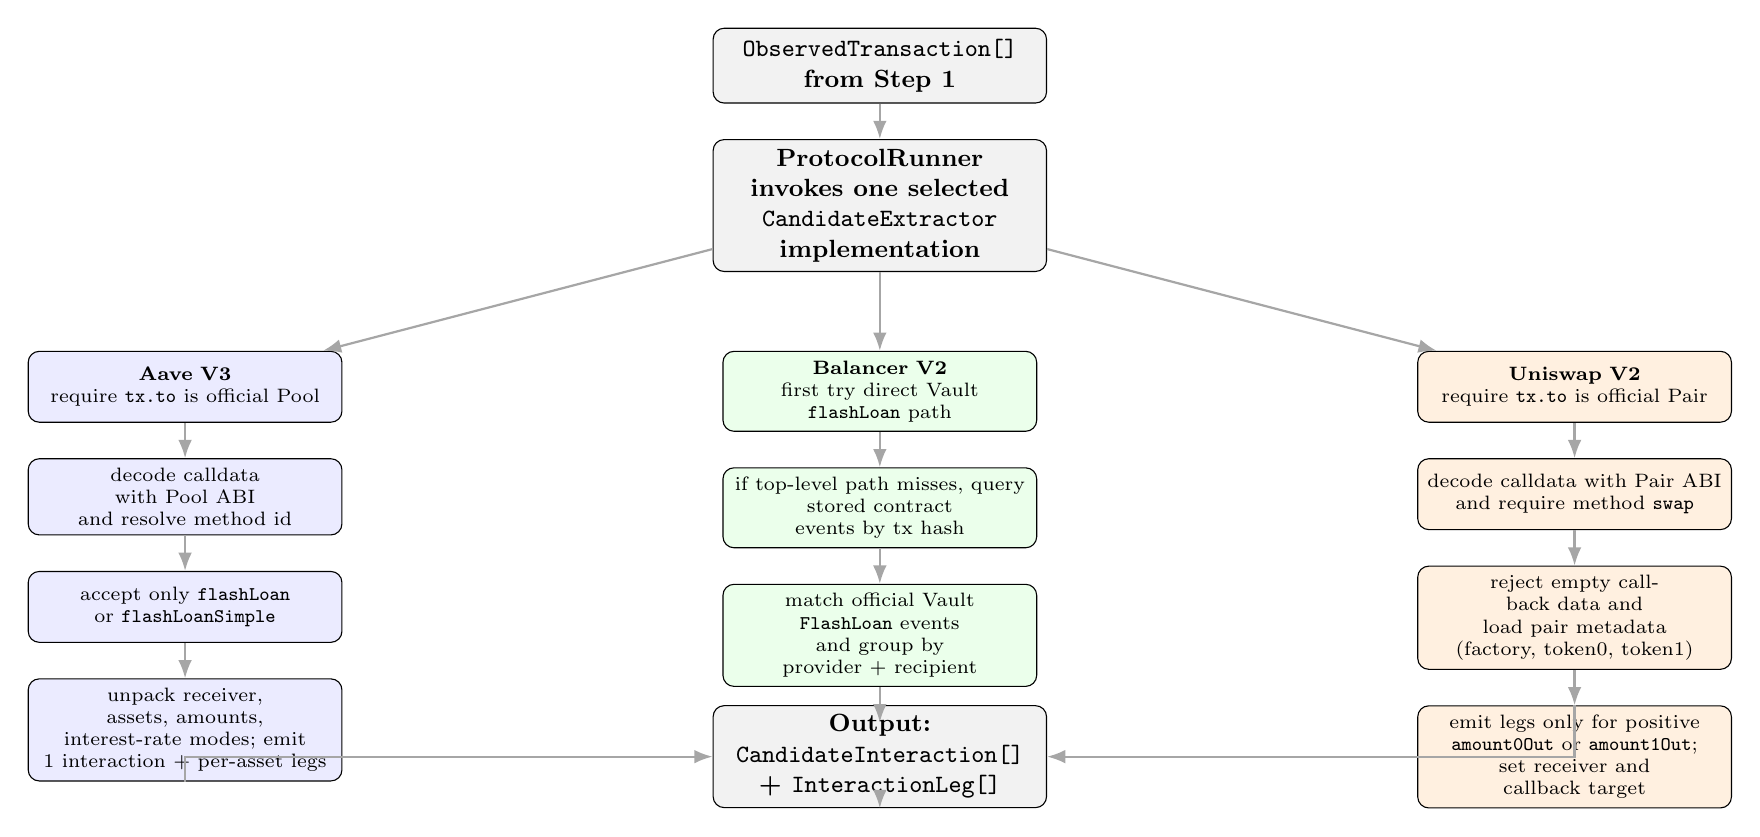
\begin{tikzpicture}[node distance=0.45cm]
  \node[head] (input) at (0,0) {\texttt{ObservedTransaction[]} from Step 1};
  \node[head, below=of input] (extractor) {ProtocolRunner invokes one selected\\\texttt{CandidateExtractor} implementation};

  \node[process, below left=1.0cm and 4.7cm of extractor] (a1) {\textbf{Aave V3}\\require \texttt{tx.to} is official Pool};
  \node[process, below=of a1] (a2) {decode calldata with Pool ABI\\and resolve method id};
  \node[process, below=of a2] (a3) {accept only \texttt{flashLoan}\\or \texttt{flashLoanSimple}};
  \node[process, below=of a3] (a4) {unpack receiver, assets, amounts,\\interest-rate modes; emit\\1 interaction + per-asset legs};

  \node[processg, below=1.0cm of extractor] (b1) {\textbf{Balancer V2}\\first try direct Vault\\\texttt{flashLoan} path};
  \node[processg, below=of b1] (b2) {if top-level path misses, query\\stored contract events by tx hash};
  \node[processg, below=of b2] (b3) {match official Vault\\\texttt{FlashLoan} events and group by\\provider + recipient};
  \node[processg, below=of b3] (b4) {emit direct or event-derived\\candidate interaction + legs\\with amount and fee fields};

  \node[processo, below right=1.0cm and 4.7cm of extractor] (u1) {\textbf{Uniswap V2}\\require \texttt{tx.to} is official Pair};
  \node[processo, below=of u1] (u2) {decode calldata with Pair ABI\\and require method \texttt{swap}};
  \node[processo, below=of u2] (u3) {reject empty callback data and\\load pair metadata\\(factory, token0, token1)};
  \node[processo, below=of u3] (u4) {emit legs only for positive\\\texttt{amount0Out} or \texttt{amount1Out};\\set receiver and callback target};

  \node[head, below=5.5cm of extractor] (output) {Output: \texttt{CandidateInteraction[]} + \texttt{InteractionLeg[]}};

  \draw[flow] (input) -- (extractor);

  \draw[flow] (extractor) -- (a1);
  \draw[flow] (extractor) -- (b1);
  \draw[flow] (extractor) -- (u1);

  \draw[flow] (a1) -- (a2);
  \draw[flow] (a2) -- (a3);
  \draw[flow] (a3) -- (a4);
  \draw[flow] (b1) -- (b2);
  \draw[flow] (b2) -- (b3);
  \draw[flow] (b3) -- (b4);
  \draw[flow] (u1) -- (u2);
  \draw[flow] (u2) -- (u3);
  \draw[flow] (u3) -- (u4);

  \draw[flow] (a4) |- (output);
  \draw[flow] (b4) -- (output);
  \draw[flow] (u4) |- (output);
\end{tikzpicture}
\end{document}
